\chapter{Чёрные дыры, белые дыры и глобальная причинная диаграмма}

\lectureoverview{Горизонт локально ничем не примечателен, но глобально имеет решающее значение. Мы начинаем с метрики Шварцшильда вблизи горизонта, затем прослеживаем её наружу с помощью аналогии с евклидовой сигарой, а после этого спрашиваем, что в действительности могут увидеть Алиса и Боб. Сингулярность и обращённая по времени область белой дыры расширяют эту локальную картину до вечного пространства-времени Шварцшильда. Компактификация Пенроуза делает причинную структуру конечной и наглядной. На последнем шаге мы переходим от вечного решения к чёрной дыре, образованной коллапсом, где теорема Ньютона об оболочке и теорема Биркгофа дают части, которые предстоит сшить.}

\section{От горизонта к бесконечности}

Вблизи достаточно большого горизонта Шварцшильда кривизна в масштабах небольшой лаборатории слаба, и геометрия в радиально-временном секторе приближённо плоская. Удобной радиальной переменной служит не координата Шварцшильда \(r\), а собственное расстояние \(\rho\), отсчитываемое наружу от горизонта вдоль пространственного сечения при постоянном времени:
\begin{equation}
\rho=0 \quad\Longleftrightarrow\quad r=2GM .
\label{eq:l04-rho-horizon}
\end{equation}
Удобной временной координатой служит безразмерная величина
\begin{equation}
\omega=\frac{t}{4GM},
\label{eq:l04-omega}
\end{equation}
где \(c=1\). Таким образом, \(\omega\) — это время Шварцшильда, измеренное в единицах удвоенного радиуса Шварцшильда.

При соглашении о сигнатуре с преобладанием плюсов пригоризонтная радиально-временная метрика имеет вид
\begin{equation}
ds^2\approx-\rho^2d\omega^2+d\rho^2.
\label{eq:l04-rindler}
\end{equation}
Угловая двусфера опущена, поскольку в данном рассуждении важны только время и радиальное расстояние.

\begin{figure}[htbp]
\centering
\includegraphics[width=0.72\textwidth]{lecture_04_figure_02.png}
\caption{Пригоризонтная метрика и перемасштабированное время Шварцшильда.}
\lectureframe{00:05:46.800}
\end{figure}

Уравнение~\eqref{eq:l04-rindler} связано с пространством-временем Минковского так же, как полярные координаты — с евклидовой плоскостью. При
\begin{equation}
T=\rho\sinh\omega,
\qquad
X=\rho\cosh\omega,
\end{equation}
получаем
\begin{equation}
-dT^2+dX^2=-\rho^2d\omega^2+d\rho^2.
\end{equation}
Линии с постоянным \(\rho\) — это гиперболы \(X^2-T^2=\rho^2\), тогда как \(\omega\) меняется от далёкого прошлого к далёкому будущему. Две нулевые линии \(X=\pm T\) встречаются в точке бифуркации редуцированной диаграммы. В четырёх измерениях этой точке соответствует двусфера, а будущая и прошлая нулевые гиперповерхности образуют бифуркатный горизонт Киллинга.\editorialnote{Называть бифуркатным горизонтом только точку пересечения — полезное сокращение на радиальной диаграмме. Точнее, две ветви горизонта пересекаются на бифуркационной двусфере.}

\subsection{Дальняя область}

Радиально-временная часть метрики Шварцшильда имеет вид
\begin{equation}
ds^2
=-\left(1-\frac{2GM}{r}\right)dt^2
+\frac{dr^2}{1-\frac{2GM}{r}}.
\label{eq:l04-schwarzschild}
\end{equation}
Вдали от дыры, \(r\gg2GM\), метрика приближается к
\begin{equation}
ds^2\approx-dt^2+dr^2.
\end{equation}
Там \(r\) и \(\rho\) отличаются лишь несущественной аддитивной поправкой, поэтому с учётом \(dt=4GM\,d\omega\)
\begin{equation}
ds^2\approx-(4GM)^2d\omega^2+d\rho^2.
\label{eq:l04-far}
\end{equation}
Радиальный коэффициент прост в обоих предельных случаях. Меняется именно временной коэффициент:
\begin{equation}
ds^2\approx
\begin{cases}
-\rho^2d\omega^2+d\rho^2, & \rho\ll GM,\\[3pt]
-(4GM)^2d\omega^2+d\rho^2, & \rho\gg GM.
\end{cases}
\label{eq:l04-two-limits}
\end{equation}
Для траектории зависания \(d\rho=0\). Вблизи горизонта
\begin{equation}
d\tau=\rho\,d\omega,
\end{equation}
тогда как вдали \(d\tau\approx4GM\,d\omega=dt\). При фиксированном приращении внешней временной координаты на часах, удерживаемых всё ближе к горизонту, проходит всё меньше собственного времени.

\subsection{Сигара}

Пространство-время трудно представить наглядно, поэтому заменим времениподобное направление обычным угловым направлением. Запишем
\begin{equation}
\begin{aligned}
d\ell^2&=F(\rho)^2d\theta^2+d\rho^2,\\
F(\rho)&\sim
\begin{cases}
\rho, & \rho\to0,\\
4GM, & \rho\to\infty.
\end{cases}
\end{aligned}
\label{eq:l04-cigar}
\end{equation}
При \(\rho=0\) это плоскость в полярных координатах. Вдали длина окружности уже не растёт с радиусом:
\begin{equation}
C_\infty=\int_0^{2\pi}4GM\,d\theta=8\pi GM.
\label{eq:l04-cigar-circumference}
\end{equation}
Поэтому поверхность закругляется на одном конце и приближается к цилиндру на другом. Она похожа на сигару.

\begin{figure}[htbp]
\centering
\includegraphics[width=0.74\textwidth]{lecture_04_figure_03.png}
\caption{Евклидово сравнение: полярное острие, соединённое с асимптотическим цилиндром длины окружности \(8\pi GM\).}
\lectureframe{00:14:05.000}
\end{figure}

Чем больше масса, тем больше асимптотический обхват и тем слабее изгиб у острия. Малой дыре соответствует сильно искривлённая сигара; у большой дыры острие широкое и слабо искривлённое. Это иллюстрация интерполяции в уравнении~\eqref{eq:l04-two-limits}, а не вложение самой лоренцевой чёрной дыры.\editorialnote{Точный геометрический объект получается аналитическим продолжением времени Шварцшильда к мнимому времени. Гладкость в острие тогда фиксирует период евклидова времени равным \(8\pi GM\) — тот же масштаб позже определяет температуру Хокинга. Здесь в лекции используется только наглядная аналогия.}

\section{Причинное истолкование горизонта}

Вне дыры, \(\rho>0\), стационарный наблюдатель движется по гиперболе с постоянным \(\rho\). Вдали требуется лишь умеренное ускорение, чтобы противостоять гравитации; вблизи горизонта необходимое собственное ускорение неограниченно растёт. Как только мировая линия пересекает будущую нулевую границу, никакой направленный в будущее причинный сигнал от неё не может достичь внешней области.

\begin{classroomqa}
\audiencequestion{Являются ли световые лучи на этой диаграмме прямыми линиями?\lecturetimestamp{00:20:21}}
\lecturerresponse{Радиальные световые лучи изображаются под углом \(45^\circ\), если не оговорено иное. Входящий луч пересекает горизонт; исходящий луч, уже находящийся внутри, не может пересечь его обратно во внешнюю область.}
\end{classroomqa}

\begin{classroomqa}
\audiencequestion{Остаётся ли входящий световой луч на горизонте?\lecturetimestamp{00:21:12}}
\lecturerresponse{Нет. Луч, направленный внутрь, пересекает будущий горизонт и продолжает путь во внутреннюю область чёрной дыры. Только сама образующая горизонта остаётся на нулевой границе.}
\end{classroomqa}

\subsection{Боб наблюдает Алису}

Пусть Боб зависает снаружи на фиксированном радиусе, а Алиса падает внутрь. Боб видит Алису, только принимая идущий от неё наружу свет. Предположим, по своим собственным часам она подаёт периодические сигналы. Сигналам, испущенным позже в ходе её падения, требуется всё больше шварцшильдова времени, чтобы достичь Боба, и он получает всё меньше таких сигналов в единицу времени. Ни один сигнал, испущенный после пересечения горизонта, не может вернуться к нему.

Координаты Риндлера делают предельное поведение явным. Определим исходящую нулевую координату
\begin{equation}
U=T-X=-\rho e^{-\omega}.
\end{equation}
Приближение к будущему горизонту означает \(U\to0^{-}\), что требует \(\omega\to+\infty\) при фиксированном внешнем \(\rho\). Поэтому событие пересечения для Алисы отодвигается на бесконечное внешнее время. Последовательные гребни волны приходят с экспоненциально растущими интервалами, поэтому их частота экспоненциально красно смещается.\editorialnote{Этот расчёт в нулевых координатах даёт математическую форму красного смещения, качественно описанного на занятии. Он использует только локальное риндлеровское приближение.}

Сначала Боб принимает свет видимого диапазона, затем инфракрасное излучение, затем радиоволны огромной длины. Содержательное утверждение не в том, что Алиса остаётся на горизонте как навсегда видимая фотография. Она становится тусклее, краснее и в конце концов необнаружимой.

\begin{classroomqa}
\audiencequestion{Видит ли Боб Алису застывшей в одном точно определённом месте вне горизонта?\lecturetimestamp{00:26:31}}
\lecturerresponse{В классическом описании на внешних координатах изображения, принимаемые во всё более поздние моменты, происходят от событий, лежащих всё ближе к горизонту. Предельное изображение там застывает, но его излучение испытывает красное смещение, пока практически не исчезает. Квантовая физика чёрных дыр в это описание ещё не входит.}
\end{classroomqa}

\begin{classroomqa}
\audiencequestion{По мере того как Алиса тускнеет, выглядит ли она также сжатой?\lecturetimestamp{00:28:34}}
\lecturerresponse{Да. Относительное движение вызывает во внешнем описании продольное лоренцево сокращение. Важнейший наблюдательный эффект здесь всё же красное смещение: её внутренние колебания кажутся более медленными, а принимаемая длина волны растёт.}
\end{classroomqa}

\subsection{Алиса наблюдает Боба}

Собственное время Алисы остаётся регулярным на горизонте. Она продолжает принимать идущие внутрь сигналы от Боба и после пересечения, поскольку эти сигналы следуют в том же причинном направлении, что и она. Оказавшись внутри, она уже не может ответить во внешнюю область. Горизонт односторонний, а не стена, встречаемая симметрично с обеих сторон.

\begin{classroomqa}
\audiencequestion{Видит ли Алиса, падая сквозь горизонт, свет Боба смещённым в синюю сторону?\lecturetimestamp{00:30:29}}
\lecturerresponse{В используемой картине она видит, что Боб удаляется, а его сигналы смещены в красную сторону; при её пересечении ничего сингулярного не происходит. Точное смещение частоты зависит и от обеих мировых линий, и от того, когда Боб испускает сигнал, поэтому инвариантное утверждение состоит в том, что измеряемая ею частота остаётся конечной на регулярном горизонте.}
\end{classroomqa}

\begin{classroomqa}
\audiencequestion{Применяется ли то же причинное ограничение к гравитонам?\lecturetimestamp{00:31:15}}
\lecturerresponse{Оно относится к подлинному гравитационному излучению так же, как и к фотонам. Никакое излучательное возмущение, испущенное из-за будущего горизонта, не может достигнуть Боба.}
\end{classroomqa}

\begin{classroomqa}
\audiencequestion{Когда Алиса падает внутрь, увеличивает ли её энергия массу и радиус дыры?\lecturetimestamp{00:31:43}}
\lecturerresponse{Да. После того как её энергия включается в чёрную дыру, её масса возрастает, и вместе с ней увеличивается её радиус Шварцшильда \(R_s=2GM\). В задаче о динамическом образовании это утверждение приобретёт геометрический смысл.}
\end{classroomqa}

\subsection{Почему во внешней области по-прежнему есть гравитация}

Чёрная дыра тёмная, но не лишена гравитации. Стационарное гравитационное поле — это не поток реальных гравитонов, непрерывно вылетающих из внутренней области. Это уже установившаяся геометрия внешней области. Если источник меняется, изменение поля распространяется причинно; далёкий наблюдатель не может обнаружить это изменение раньше, чем мог бы прийти световой сигнал.

\begin{classroomqa}
\audiencequestion{Если гравитоны не могут вырваться наружу, почему чёрная дыра вообще оказывает гравитационное воздействие?\lecturetimestamp{00:32:04}}
\lecturerresponse{Статическое поле уже присутствует снаружи. Его можно вольно описывать через виртуальные гравитоны, но это не детектируемые частицы, несущие новые сигналы изнутри. Скоростью света ограничено изменение поля, включая гравитационное излучение.}
\end{classroomqa}

\begin{classroomqa}
\audiencequestion{Как согласовать виртуальные гравитоны с утверждением, что изменение поля распространяется со скоростью света?\lecturetimestamp{00:34:02}}
\lecturerresponse{Виртуальные кванты — это элементы учёта в пертурбативном вычислении, а не частицы, несущие сигнал, с измеримыми траекториями. Калибровочно-инвариантные возмущения и информация распространяются причинно. То же различие возникает между статическим электромагнитным полем и электромагнитным излучением.}
\end{classroomqa}

Поэтому учебную формулировку о том, что виртуальные гравитоны могут превышать скорость света, не следует понимать как сверхсветовую передачу информации.\editorialnote{Виртуальные частицы вне массовой оболочки не обязаны удовлетворять дисперсионному соотношению на массовой оболочке, но они не являются наблюдаемыми и не могут использоваться для передачи информации. В общей теории относительности есть более ясное и простое описание: существует стационарная внешняя метрика, тогда как изменения гравитационного поля распространяются причинно.}

\section{Может ли Алиса всё ещё видеть свои ноги?}

Пусть Алиса падает ногами вперёд. Её ноги пересекают горизонт раньше головы. Когда она смотрит вниз, она никогда не видит одновременное событие на мировой линии своих ног; свету нужно время на распространение, поэтому она видит свои ноги в немного более раннем событии. Непрерывная последовательность таких прошлых событий существует и до, и после того, как её голова пересекает горизонт. Ничего локально разрывного не происходит лишь потому, что одна часть её тела прошла \(r=2GM\).

Опасный эксперимент состоит в том, чтобы развернуться после того, как ноги оказались внутри. Чтобы удержать голову снаружи, Алиса должна ускоряться наружу. Её ноги, уже находящиеся за будущим горизонтом, не могут следовать траектории зависания во внешней области. В ускоренной системе отсчёта разделение растёт без границ, и материальное тело не может оставаться жёстким через эту причинную границу. Она должна либо свободно падать вместе со своими ногами, либо быть разорванной, пытаясь удержать остальную часть себя снаружи.

Это растяжение не является расходящейся приливной силой на большом горизонте. Оно является следствием требования несовместимых мировых линий для протяжённого тела.\editorialnote{У достаточно большого горизонта Шварцшильда приливная кривизна мала. Патология в этом мысленном эксперименте возникает из-за попытки ускорения и условия жёсткости, а не из-за локальной сингулярности кривизны на горизонте.}

\section{Сингулярность находится в будущем}

Вернёмся к уравнению~\eqref{eq:l04-schwarzschild}. Снаружи,
\begin{equation}
1-\frac{2GM}{r}>0,
\end{equation}
поэтому координата \(t\) является времениподобной, а \(r\) — пространственноподобной в координатах Шварцшильда. Внутри,
\begin{equation}
1-\frac{2GM}{r}<0,
\end{equation}
и эти координатные роли меняются местами: убывание \(r\) задаёт времениподобное направление. Это не означает, что на горизонте пространство физически превращается во время. Это означает, что там координатная карта Шварцшильда вырождается и что внутри её метки имеют иной причинный характер.

Подлинная сингулярность находится при
\begin{equation}
r=0.
\end{equation}
Это не вертикальная мировая линия, представляющая место, которого можно было бы избежать. Это пространственноподобная будущая граница. Как только Алиса входит в область чёрной дыры, каждая направленная в будущее времениподобная или светоподобная кривая заканчивается там. Инвариант кривизны
\begin{equation}
R_{\mu\nu\rho\sigma}R^{\mu\nu\rho\sigma}
=\frac{48G^2M^2}{r^6}
\label{eq:l04-kretschmann}
\end{equation}
расходится при \(r\to0\), тогда как при \(r=2GM\) он конечен.\editorialnote{Уравнение~\eqref{eq:l04-kretschmann} — это стандартный скаляр Кречмана для решения Шварцшильда. Оно придаёт инвариантный смысл различию, геометрически проведённому на лекции, между регулярным горизонтом и сингулярностью кривизны.}

\section{Обращение времени и белая дыра}

Метрика Шварцшильда не зависит от \(t\), а \(dt^2\) не меняется при \(t\mapsto-t\). Поэтому её максимальное продолжение симметрично относительно обращения времени. Наряду с будущей сингулярностью и будущим горизонтом математическое решение содержит прошлую сингулярность и прошлый горизонт.

Обратим по времени падение Алисы. Теперь она выходит из прошлой сингулярности, пересекает прошлый горизонт наружу и появляется во внешней области Боба. Эта область называется белой дырой. Это не путь выхода из будущей внутренней области чёрной дыры: будущий и прошлый горизонты — разные светоподобные границы.

\begin{classroomqa}
\audiencequestion{Если Алиса не может пересечь горизонт чёрной дыры наружу, как тогда обращённая по времени Алиса может выйти?\lecturetimestamp{00:50:24}}
\lecturerresponse{Она не пересекает будущий горизонт наружу. Она пересекает прошлый горизонт наружу, в точности как при обращении времени обычного падения. В будущей области чёрной дыры по-прежнему нет причинного пути наружу.}
\end{classroomqa}

\begin{classroomqa}
\audiencequestion{Нужно ли в картине белой дыры также прокручивать всю историю Боба в обратном направлении?\lecturetimestamp{00:52:15}}
\lecturerresponse{Нет. Расширенная геометрия допускает историю, в которой Боб остаётся во внешней области, тогда как Алиса выходит из прошлого горизонта. Проблема не в математической непротиворечивости; она в чрезвычайно необычном начальном условии, представленном прошлой сингулярностью.}
\end{classroomqa}

\begin{figure}[htbp]
\centering
\includegraphics[width=0.72\textwidth]{lecture_04_figure_04.png}
\caption{Развёрнутый причинный эскиз: пересекающиеся горизонты, кривые будущей и прошлой сингулярностей и траектории наблюдателей, накопленные по ходу обсуждения.}
\lectureframe{01:00:19.818}
\end{figure}

\begin{figure}[htbp]
\centering
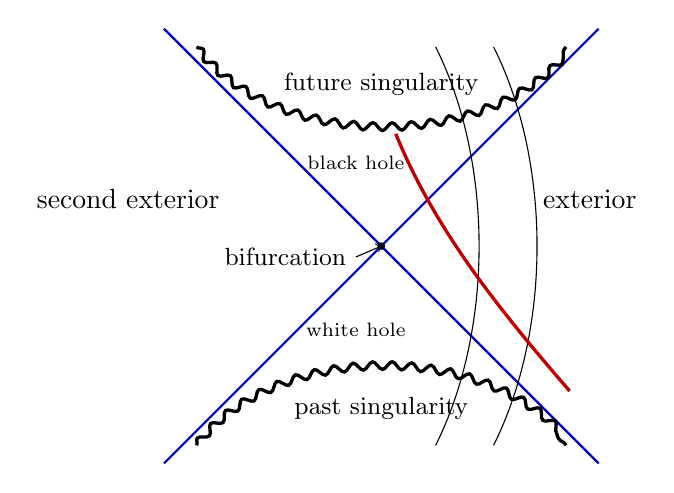
\begin{tikzpicture}[scale=0.92]
\draw[blue!75!black,thick] (-3,-3) -- (3,3);
\draw[blue!75!black,thick] (-3,3) -- (3,-3);
\draw[very thick,decorate,decoration={snake,amplitude=1.4pt,segment length=7pt}]
  (-2.55,2.75) .. controls (-1.45,1.35) and (1.45,1.35) .. (2.55,2.75);
\draw[very thick,decorate,decoration={snake,amplitude=1.4pt,segment length=7pt}]
  (-2.55,-2.75) .. controls (-1.45,-1.35) and (1.45,-1.35) .. (2.55,-2.75);
\draw (0.75,-2.75) .. controls (1.55,-1.15) and (1.55,1.15) .. (0.75,2.75);
\draw (1.55,-2.75) .. controls (2.35,-1.15) and (2.35,1.15) .. (1.55,2.75);
\draw[red!75!black,very thick] (2.6,-2.0) .. controls (1.65,-0.9) and (0.75,0.2) .. (0.2,1.55);
\fill (0,0) circle (1.5pt);
\node[above,font=\small] at (0,1.95) {future singularity};
\node[below,font=\small] at (0,-1.95) {past singularity};
\node[right] at (2.10,0.65) {exterior};
\node[left] at (-2.10,0.65) {second exterior};
\node[font=\scriptsize] at (-0.35,1.15) {black hole};
\node[font=\scriptsize] at (-0.35,-1.15) {white hole};
\node[font=\small,anchor=east] (bifurcation-label) at (-0.35,-0.15) {bifurcation};
\draw[->,thin] (bifurcation-label.east) -- (0,0);
\end{tikzpicture}
\caption{Очищенная некомпактифицированная причинная картина. Светоподобные горизонты пересекаются на бифуркационной поверхности; пространственноподобные сингулярности лежат в будущей и прошлой клиновидных областях.}
\end{figure}

\subsection{Возможное не типично}

Микроскопическая механика с превосходной точностью инвариантна относительно обращения времени, однако у макроскопических процессов есть предпочтённое направление. Бомба легко взрывается; разлетевшиеся осколки почти никогда вновь не собираются, чтобы восстановить её. Шар легко скатывается с неустойчивой вершины; случайно брошенный шар почти никогда не останавливается точно на ней. Бильярдные шары, собранные в треугольник, легко разлетаются, тогда как разрозненные шары самопроизвольно не выстраиваются в такой треугольник. Кубик льда тает в горячей воде, тогда как вода почти никогда не выталкивает из себя заново собранный кубик льда.

Различие определяется энтропией. Макросостояние с низкой энтропией занимает крошечную область фазового пространства; макросостояние с высокой энтропией содержит огромное число микроскопических конфигураций. Уравнения допускают обращённую траекторию, но подготовка её начального микросостояния требует фантастически точных корреляций.

\begin{classroomqa}
\audiencequestion{Разве каждая точная разлетевшаяся конфигурация не столь же маловероятна, как и точная обращённая по времени?\lecturetimestamp{00:56:55}}
\lecturerresponse{Да, если речь идёт об индивидуально заданных микросостояниях. Асимметрия появляется, когда мы сравниваем макросостояния. Разлетевшаяся конфигурация включает несравненно больше микросостояний, чем точно собранный треугольник, поэтому почти всякое микросостояние, совместимое с первым описанием, остаётся макроскопически неупорядоченным.}
\end{classroomqa}

Белая дыра, испускающая полностью организованную Алису, — это гравитационная версия такой истории с понижением энтропии. Она разрешена обратимыми уравнениями, но требует чрезвычайно специального прошлого. Сам горизонт несёт энтропию и скрытую микроскопическую информацию, поэтому флуктуация масштаба Алисы логически не запрещена; она крайне сильно подавлена.

\begin{classroomqa}
\audiencequestion{Была бы такая флуктуация квантовомеханической или тепловой?\lecturetimestamp{00:59:48}}
\lecturerresponse{Могут вносить вклад оба типа. В обычной горячей системе естественнее говорить о тепловой флуктуации; для чёрной дыры квантовые и тепловые эффекты переплетены. В любом случае основное подавление носит энтропийный характер.}
\end{classroomqa}

\section{Собственное расстояние и компактификация Пенроуза}

Прежде чем рисовать глобальную картину пространства-времени, следует уточнить радиальную терминологию. Собственное время — это то, что часы измеряют вдоль времениподобной мировой линии. Собственное расстояние — это то, что цепочка локальных мерных стержней измеряет вдоль выбранной пространственноподобной кривой. Для шварцшильдова среза при постоянном \(t\),
\begin{equation}
d\rho=\frac{dr}{\sqrt{1-2GM/r}}.
\label{eq:l04-proper-distance}
\end{equation}
Следовательно, \(r\) — это ареальная координата, а не прямое расстояние по линейкам до горизонта.

Теперь начнём с радиального плоского пространства-времени. Оставим только \(t\) и \(\rho\ge0\). Прямая \(\rho=0\) — это пространственное начало координат, и радиальный световой луч, входящий в начало, продолжает идти наружу по противоположной физической стороне, что в редуцированной полуплоскости выглядит как отражение.

Диаграмма Пенроуза отображает все конечные и бесконечные значения \(t\) и \(\rho\) в конечную область, сохраняя при этом светоподобные направления. Её два правила таковы:
\begin{enumerate}
\item скомпактифицировать всё пространство-время в конечную область;
\item сохранять радиальные световые лучи под углом \(45^\circ\).
\end{enumerate}
Длины и обычные углы искажаются; причинные соотношения — нет.

\begin{figure}[htbp]
\centering
\includegraphics[width=0.70\textwidth]{lecture_04_figure_06.png}
\caption{Завершённая сетка компактификации для радиального пространства-времени Минковского. Бесконечное время находится в левой верхней и левой нижней крайних точках, а бесконечный радиус сжат до правой вершины.}
\lectureframe{01:14:44.040}
\end{figure}

\begin{figure}[htbp]
\centering
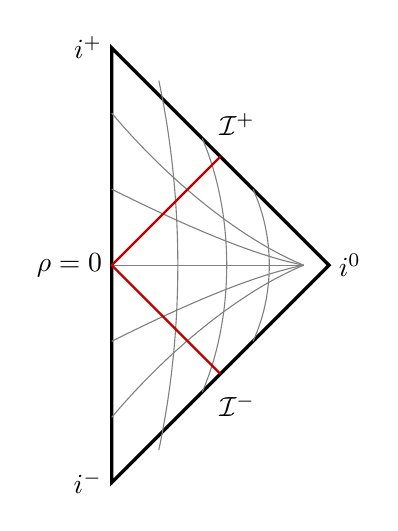
\begin{tikzpicture}[scale=0.92]
\coordinate (im) at (0,-3);
\coordinate (ip) at (0,3);
\coordinate (iz) at (3,0);
\draw[very thick] (im) -- (ip) -- (iz) -- cycle;
\draw[gray] (0,-2.1) .. controls (0.8,-1.15) and (1.8,-0.35) .. (2.65,0);
\draw[gray] (0,-1.05) .. controls (0.9,-0.6) and (1.9,-0.15) .. (2.65,0);
\draw[gray] (0,0) -- (2.65,0);
\draw[gray] (0,1.05) .. controls (0.9,0.6) and (1.9,0.15) .. (2.65,0);
\draw[gray] (0,2.1) .. controls (0.8,1.15) and (1.8,0.35) .. (2.65,0);
\draw[gray] (0.65,-2.55) .. controls (1.0,-0.9) and (1.0,0.9) .. (0.65,2.55);
\draw[gray] (1.25,-1.75) .. controls (1.7,-0.7) and (1.7,0.7) .. (1.25,1.75);
\draw[gray] (1.95,-1.05) .. controls (2.25,-0.4) and (2.25,0.4) .. (1.95,1.05);
\draw[red!75!black,thick] (1.5,-1.5) -- (0,0) -- (1.5,1.5);
\node[left] at (ip) {\(i^+\)};
\node[left] at (im) {\(i^-\)};
\node[right] at (iz) {\(i^0\)};
\node[above right] at (1.35,1.65) {\(\mathcal{I}^+\)};
\node[below right] at (1.35,-1.65) {\(\mathcal{I}^-\)};
\node[left] at (0,0) {\(\rho=0\)};
\end{tikzpicture}
\caption{Радиальная часть пространства-времени Минковского в виде конечного треугольника. Красный светоподобный луч входит из \(\mathcal{I}^-\), достигает начала и выходит через \(\mathcal{I}^+\).}
\label{fig:l04-flat-penrose}
\end{figure}

Конечные точки имеют различный причинный смысл:
\begin{equation}
\begin{aligned}
i^-&:\ \text{past timelike infinity},\\
i^+&:\ \text{future timelike infinity},\\
i^0&:\ \text{spatial infinity},\\
\mathcal{I}^-&:\ \text{past null infinity},\\
\mathcal{I}^+&:\ \text{future null infinity}.
\end{aligned}
\end{equation}
Символы \(\mathcal{I}^{-}\) и \(\mathcal{I}^{+}\) произносятся как скрай минус и скрай плюс.

\begin{classroomqa}
\audiencequestion{Должен ли светоподобный луч проходить через углы каждой искажённой ячейки сетки и потому слегка искривляться?\lecturetimestamp{01:11:08}}
\lecturerresponse{Если бы полная координатная сетка была нарисована точно, её пересечения согласовывались бы со светоподобной кривой. Существенно здесь то, что построение конформно: радиальные светоподобные направления остаются под углом \(45^\circ\), хотя линии постоянного \(t\) и постоянного \(\rho\) изгибаются и сгущаются.}
\end{classroomqa}

\begin{classroomqa}
\audiencequestion{Как изображается световой луч, если он не проходит через начало?\lecturetimestamp{01:11:45}}
\lecturerresponse{Он достигает ненулевого расстояния наибольшего сближения и затем возвращается наружу. При учёте углового движения его радиальная проекция не обязана быть одной прямой линией под углом \(45^\circ\).}
\end{classroomqa}

\begin{classroomqa}
\audiencequestion{Тогда почему этот световой луч не идёт под углом \(45^\circ\)?\lecturetimestamp{01:12:49}}
\lecturerresponse{Правило про \(45^\circ\) было сформулировано для радиальных световых лучей. Светоподобный луч с угловым моментом тратит часть своего движения на угловые направления, так что его проекция на плоскость \(t\)-\(\rho\) не является радиальной.}
\end{classroomqa}

\section{Вечная диаграмма Шварцшильда}

Компактифицированная диаграмма имеет четыре области. Её два боковых ромба — асимптотически плоские внешние области. Верхний треугольник — внутренняя область чёрной дыры, оканчивающаяся на будущей пространственноподобной сингулярности. Нижний треугольник — область белой дыры, начинающаяся на прошлой пространственноподобной сингулярности. Вместе эти области образуют максимально продолженную геометрию Шварцшильда.

\begin{figure}[htbp]
\centering
\includegraphics[width=0.74\textwidth]{lecture_04_figure_07.png}
\caption{Полная диаграмма Пенроуза для вечного решения Шварцшильда; на доске отмечены сингулярности, горизонты, светоподобные траектории и одна асимптотическая граница.}
\lectureframe{01:21:30.000}
\end{figure}

\begin{figure}[htbp]
\centering
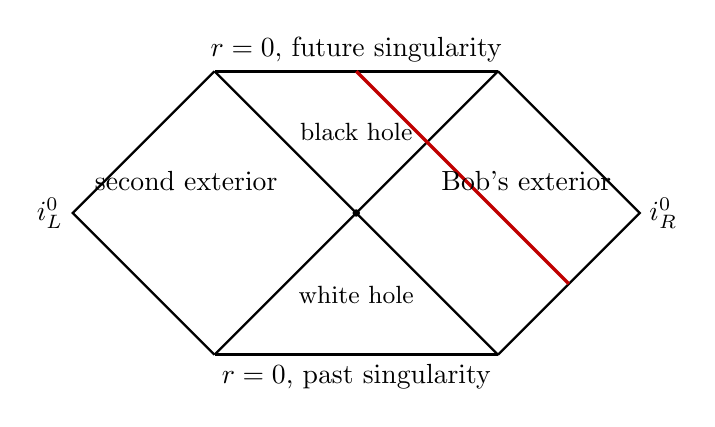
\begin{tikzpicture}[scale=0.90]
\coordinate (C) at (0,0);
\coordinate (TL) at (-2,2);
\coordinate (TR) at (2,2);
\coordinate (BL) at (-2,-2);
\coordinate (BR) at (2,-2);
\coordinate (L) at (-4.0,0);
\coordinate (R) at (4.0,0);
\draw[very thick] (TL) -- (TR);
\draw[very thick] (BL) -- (BR);
\draw[thick] (C) -- (TL) (C) -- (TR) (C) -- (BL) (C) -- (BR);
\draw[thick] (TL) -- (L) -- (BL);
\draw[thick] (TR) -- (R) -- (BR);
\draw[red!75!black,very thick] (3,-1) -- (1,1) -- (0,2);
\node[above] at (0,2) {\(r=0\), future singularity};
\node[below] at (0,-2) {\(r=0\), past singularity};
\node[font=\small] at (0,1.15) {black hole};
\node[font=\small] at (0,-1.15) {white hole};
\node at (2.4,0.45) {Bob's exterior};
\node at (-2.4,0.45) {second exterior};
\node[right] at (R) {\(i^0_R\)};
\node[left] at (L) {\(i^0_L\)};
\fill (C) circle (1.5pt);
\end{tikzpicture}
\caption{Четыре области вечного решения Шварцшильда. Входящий радиальный световой луч пересекает будущий горизонт и приходит к \(r=0\).}
\label{fig:l04-eternal}
\end{figure}

Входящий радиальный световой луч из \(\mathcal{I}^-\) пересекает будущий горизонт и оканчивается на сингулярности. Любая причинная кривая в верхнем треугольнике разделяет эту судьбу. Вторую внешнюю область часто описывают как другое устье моста Эйнштейна--Розена, но он непроходим: любая попытка совершить причинное путешествие из одной внешней области в другую входит в область чёрной дыры и достигает сингулярности.

\begin{classroomqa}
\audiencequestion{Соединены ли две внешние вселенные кротовой норой, и можно ли передать через неё сигнал?\lecturetimestamp{01:22:21}}
\lecturerresponse{Вечная геометрия содержит мост Эйнштейна--Розена на подходящих пространственных срезах, но ни один причинный сигнал не переходит из одной внешней области в другую. Он пережимается слишком быстро; даже свет, пересекающий горизонт, оканчивается на будущей сингулярности.}
\end{classroomqa}

Эта диаграмма описывает чёрную дыру, существовавшую всё время. Реальные астрофизические чёрные дыры образуются из коллапсирующего вещества. В их причинной диаграмме нет ни прошлой сингулярности белой дыры, ни второй асимптотической внешней области. Чтобы построить такую геометрию, нам нужно понять сферические оболочки.

\section{Формирование чёрной дыры коллапсом}

Представьте себе разреженную сферическую оболочку из входящих частиц. Ими могут быть фотоны: энергия гравитирует, так что достаточно концентрированный импульс излучения может образовать чёрную дыру. До коллапса центральная область напоминает пустое плоское пространство-время; после сжатия достаточной энергии внешняя область напоминает решение Шварцшильда. Задача состоит в том, чтобы сшить эти области по движущейся оболочке.

\subsection{Теорема Ньютона об оболочке}

Для сферически симметричной ньютоновской оболочки полной массы \(M\) закон Гаусса для гравитации имеет вид
\begin{equation}
\oint \mathbf{g}\cdot d\mathbf{A}=-4\pi G M_{\mathrm{enc}}.
\label{eq:l04-gauss-gravity}
\end{equation}
Сферическая симметрия означает, что \(\mathbf{g}=g(r)\hat{\mathbf r}\), так что
\begin{equation}
g(r)=
\begin{cases}
0, & r<R_{\mathrm{shell}},\\[4pt]
-\dfrac{GM}{r^2}, & r>R_{\mathrm{shell}}.
\end{cases}
\label{eq:l04-shell-field}
\end{equation}
Внутри заключённой массы нет, и гравитационное поле обращается в нуль. Снаружи оболочка действует в точности как точечная масса \(M\) в центре. Потенциал внутри постоянен, а не равен нулю, но никакой локальной ньютоновской силы не остаётся.\editorialnote{Аргумент через силовые линии, приведённый на занятии, точно выражается законом Гаусса. Различие между нулевым полем и постоянным потенциалом важно при сравнении нормировок часов в теории относительности.}

Этот вывод остаётся верным и при сжатии идеально сферической оболочки, если её полная масса сохраняется. Меняется только положение границы между внутренним и внешним решениями.

\subsection{Теорема Биркгофа}

Релятивистский аналог — теорема Биркгофа: всякая сферически симметричная вакуумная область локально является частью семейства решений Шварцшильда. Для оболочки, в центре которой нет массы,
\begin{align}
ds^2_{\mathrm{inside}}&=-dT^2+dR^2+R^2d\Omega_2^2,\\
ds^2_{\mathrm{outside}}&=
-\left(1-\frac{2GM}{r}\right)dt^2
\nonumber\\
&\quad+\frac{dr^2}{1-2GM/r}
+r^2d\Omega_2^2.
\label{eq:l04-birkhoff-pieces}
\end{align}

\begin{figure}[htbp]
\centering
\includegraphics[width=0.74\textwidth]{lecture_04_figure_08.png}
\caption{Схема сшивки по оболочке: внутри окружности плоское пространство-время, снаружи — решение Шварцшильда.}
\lectureframe{01:34:15.000}
\end{figure}

\begin{classroomqa}
\audiencequestion{Какая метрика возникает снаружи сферической оболочки в общей теории относительности?\lecturetimestamp{01:33:17}}
\lecturerresponse{Метрика Шварцшильда с параметром массы, равным полной сохраняемой массе оболочки. Пустая центральная область локально является пространством-временем Минковского.}
\end{classroomqa}

\begin{classroomqa}
\audiencequestion{Если оболочка сжимается, почему параметр массы не меняется?\lecturetimestamp{01:34:33}}
\lecturerresponse{Потому что полная энергия сохраняется. Радиус оболочки и кинетический вклад или вклад энергии связи могут меняться, но сохраняющаяся масса внешнего решения фиксирована для изолированной сферической системы. Движущаяся оболочка меняет то, где сшиваются плоская область и область Шварцшильда.}
\end{classroomqa}

Плоская внутренняя область не означает, что внутренние часы обязательно имеют ту же нормировку, что и часы на бесконечности. Сшивка на оболочке может умножить внутреннюю временную координату на константу, а движущаяся оболочка требует соответствующих условий склейки.\editorialnote{Теорема Биркгофа локально фиксирует каждую вакуумную область. Глобальное соотношение между их координатами определяется согласованием индуцированной метрики и внешней кривизны на оболочке. Эти подробности отложены, точно так же как и построение коллапса отложено до следующей лекции.}

Теперь у нас есть две части, необходимые для формирования: пространство-время Минковского внутри сжимающейся оболочки и пространство-время Шварцшильда вне её. По мере движения оболочки внутрь граница между ними описывает мировую трубку. Проследив эту трубку через тот радиус, который должен стать радиусом Шварцшильда, мы заменим нефизическую прошлую половину рисунка~\ref{fig:l04-eternal} регулярной доколлапсной областью и увидим, где начинается горизонт событий реальной чёрной дыры.
